\documentclass[12pt]{article}
\usepackage[english]{babel}
\usepackage[utf8x]{inputenc}
\usepackage{amsmath}
\usepackage{graphicx}
\usepackage[a4paper]{geometry}

\usepackage{listings}
\usepackage{color}

\definecolor{dkgreen}{rgb}{0,0.6,0}
\definecolor{gray}{rgb}{0.5,0.5,0.5}
\definecolor{mauve}{rgb}{0.58,0,0.82}

\lstset{frame=tb,
  language=Matlab,
  aboveskip=3mm,
  belowskip=3mm,
  showstringspaces=false,
  columns=flexible,
  basicstyle={\small\ttfamily},
  numbers=none,
  numberstyle=\tiny\color{gray},
  keywordstyle=\color{blue},
  commentstyle=\color{dkgreen},
  stringstyle=\color{mauve},
  breaklines=true,
  breakatwhitespace=true,
  tabsize=3
}

\begin{document}
\begin{titlepage}

% definition of custom command for horizontal lines
\newcommand{\HRule}{\rule{\linewidth}{0.5mm}}

\center
% HEADING
\textsc{\LARGE University of Dublin,\\Trinity College}\\[1.0cm]

\includegraphics[width=0.2\textwidth]{logo.png}

\HRule \\[0.4cm]
\textsc{\Large JS Engineering: 3C1 Signals \& Systems}\\[0.25cm]
\textsc{\large S1: Linear Time Invariant Systems}\\[0.1cm]
\HRule \\[0.4cm]
 
% AUTHORS
\begin{minipage}{0.5\textwidth}
\begin{flushleft} \large
\emph{Author:}
\\Edmond \textsc{O'Flynn} 12304742
\end{flushleft}
\end{minipage}
~
\begin{minipage}{0.4\textwidth}
\begin{flushleft} 
\large
\emph{Lecturer:} \\
William \textsc{Dowling} 
\end{flushleft}
\end{minipage}\\[6cm]

% DATE
{\large \today}\\[2cm] 

% LOGO
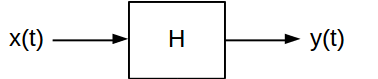
\includegraphics[width=0.5\textwidth]{lti.png}
\clearpage
\end{titlepage}

\newgeometry{top=1cm,left=1cm,bottom=2cm,right=1cm}
\tableofcontents
\addcontentsline{toc}{section}{References}
\thispagestyle{empty}
\cleardoublepage
\setcounter{page}{1}

\newgeometry{top=2cm,left=2cm,bottom=2cm,right=2cm}

\section{Abstract}

\section{Matlab}
In this laboratory, the scripting language \emph{Matlab} was used which gets compiled at its runtime. This makes for a language that is great for rapid-prototyping and extensive functionality within arithmetic, graphing, and graphical user interfaces. During this report, Matlab code snippets will be occasionally shown.

\section{Signals}
\subsection{Plotting the Deterministic Sine Wave $x_1$}
\begin{itemize}
\item Generate a deterministic signal $x_1=3sin(5t)$ over the range $0 \leq t \leq 6$ seconds.
\end{itemize}

\begin{lstlisting}
t = (0:0.01:6); % range 0-6 with steps of 0.01s
x1 = 3 * sin(5 * t);
figure(1); plot(t,x1);
title('Sine Wave Seconds v Voltages');
xlabel('Seconds (s)'); ylabel('Volts (V)');
\end{lstlisting}

\subsubsection{Properties}
\begin{itemize}
\item Voltage extrema
\begin{itemize}
\item Maximum: 3V
\item Minimum: -3V
\end{itemize}
\item Frequency
\begin{itemize}
\item 1.256s for 1 oscillation
\item $\frac{1}{1.256} \approx 0.796$Hz
\item Also determined from $\frac{5}{2\pi}$, where 5 refers to the factor before t, which also results in $0.796$ Hz
\end{itemize}
\item Periodicity
\begin{itemize}
\item Time for one cycle of the wave is 1.256s.
\end{itemize}
\end{itemize}

\subsection{Expanding to $x_2$}
\begin{itemize}
\item Generate a deterministic signal $x_2=Asin(\omega_{1}t + \phi)$ over the range $0 \leq t \leq 6$ seconds.
\end{itemize}

\begin{lstlisting}
w1 = 5;
phi = -3;
A = 3;
x2 = A * sin(w1 * t + phi);
hold on;plot(t,x2,'r');title('Sine Wave Seconds v Voltages');
xlabel('Seconds (s)');ylabel('Volts (V)');
\end{lstlisting}
Note that the same plot is overlaid using the hold on command for the plot given a previous one.

\subsubsection{Properties}
\begin{itemize}
\item Frequency
\begin{itemize}
\item 1.256s for 1 oscillation
\item $\frac{1}{1.256} \approx 0.796$Hz
\item Also determined from $\frac{5}{2\pi}$, where 5 refers to the factor before t, which also results in $0.796$ Hz
\end{itemize}
\item Periodicity
\begin{itemize}
\item Time for one cycle of the wave is 1.256s.
\end{itemize}
\item Differences between $x_1$ and $x_2$
\begin{itemize}
\item $x_1$ is a regular sine wave that has no offsets or lags. $x_2$ however, is offset such that it has almost become inverted. They two signals share the same amplitude and frequency.
\end{itemize}
\item Is there a phase lag?
\begin{itemize}
\item Yes there is. $x_2$ contains a lag $\phi$ that is not present in $x_1$.
\end{itemize}
\item Is this a delay or an advance?
\begin{itemize}
\item This is a delay with respect to $x_1$.
\end{itemize}
\end{itemize}

\subsubsection{Delay}
Between $x_2$ and $x_1$, there is about 0.657s lag time. I picked one point common to both signals (-3V), and recorded the difference in time between the two signals to reach this. 

\subsection{Expanding Further to $x_3$}
\begin{itemize}
\item Generate a deterministic signal $x_3=Asin(\omega_{1}t + \phi)$ over the range $0 \leq t \leq 6$ seconds.
\end{itemize}

\begin{lstlisting}
w1 = 5;
phi = -3 + (2 * 3.14);
A = 3;
x3 = A * sin(w1 * t + phi);
hold on;plot(t,x3,'r');title('Sine Wave Seconds v Voltages');
xlabel('Seconds (s)');ylabel('Volts (V)');
\end{lstlisting}

\subsubsection{Properties}
The function generated by $x_3$ is identical to $x_2$. The only difference is that $x_3$ has been shifted by $2\pi$, thus they are in phase with one another, and overlay accordingly.
\section{Linear Time Invariant Systems}
\subsection{LTI Systems}
\subsubsection{Input vs Output}
\begin{itemize}
\item Input v Output
\begin{itemize}
\item Both of the input and output signals of system 1 are sine waves. The output takes a few cycles to reach a steady state with amplitude varying accordingly.
\end{itemize}
\end{itemize}
\subsubsection{Differences between Signals}
\begin{itemize}
\item What are the differences between the input and output signals using system 1?
\begin{itemize}
\item The difference between the input and output lies with an approximate 0.08s delay with respect to the input. The frequencies remain the same though, while the amplitude initially overshoots and then decays to a steady state amplitude that is lower than the input's amplitude voltage after some cycles have elapsed.
\end{itemize}
\item What is the same?
\begin{itemize}
\item The sine transient input has remained the same.
\end{itemize}
\end{itemize}
\subsubsection{2x Amplitude Factors}
\begin{itemize}
\item What is the corresponding increase in the output signal amplitude given that its initial transients have decayed?
\begin{itemize}
\item The amplitude of the output signal is approximately 3.71V where the input signal's amplitude is 4V.
\end{itemize}
\item How long does the system take to settle into a steady state response?
\begin{itemize}
\item After approximately 0.325s the system has entered a steady state.
\end{itemize}
\end{itemize}
\subsubsection{Relationship between Factors}
\begin{itemize}
\item Given input amplitudes $0.5,1.0\quad...\quad2.5$, measure the corresponding output amplitudes
\begin{itemize}
\item Given the range of amplitudes, the following table and graph show the linear effect of amplitude vs output:
\end{itemize}
\end{itemize}
\begin{table}[h]
\centering
\begin{tabular}{ll}
Input (V) & Output (V) \\
0.5       & 0.47       \\
1.0       & 0.93        \\
1.5       & 1.4       \\
2.0       & 1.87        \\
2.5       & 2.34      
\end{tabular}
\caption{Input vs Output Voltages}
\end{table}

\begin{align*}
\centering
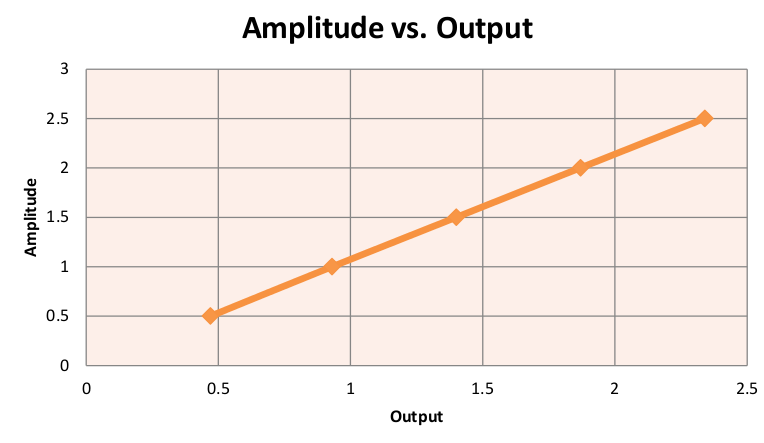
\includegraphics[width=0.7\textwidth]{amp_v_output.png}
\end{align*}

\subsubsection{Cosine Waves in System 1}
\begin{itemize}
\item What is the difference between the input and output signals using system 1?
\begin{itemize}
\item The difference between the outputa dn the intput signals is that the output signal's amplitude value is again higher than the input signal's one, where the amplitude of the output signal is now $\approx1.87V$ and the input is $2V$.
\end{itemize}
\item What is the same?
\begin{itemize}
\item The output signal is shifted to the right of the input signal by $\approx0.06$s, as seen in the images.
\end{itemize}
\end{itemize}
\begin{table}[h]
\centering
\begin{tabular}{ll}
Input (V) & Output (V) \\
0.5       & 0.75       \\
1.0       & 1.5        \\
1.5       & 2.25       \\
2.0       & 3.0        \\
2.5       & 3.75      
\end{tabular}
\caption{Input vs Output Voltages}
\end{table}
\begin{align*}
\centering
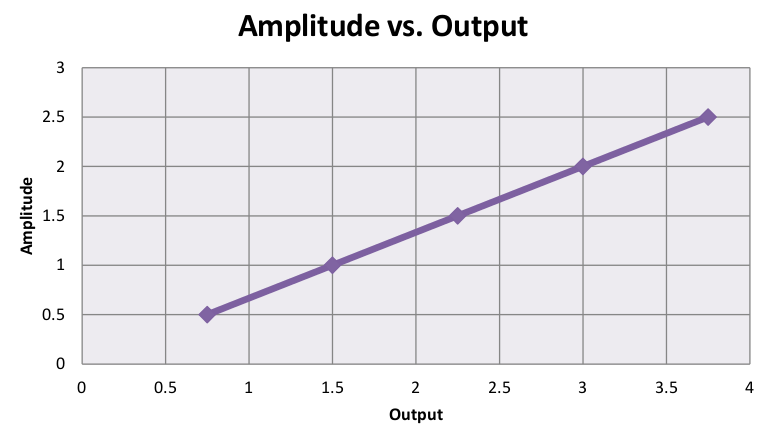
\includegraphics[width=0.7\textwidth]{amp_v_output_2.png}
\end{align*}
\subsubsection{Mathematical Approximation}
\begin{itemize}
\item For both the sine and cosine functions with frequency 2Hz and amplitude 2 under system 1, approximate expressions for input and output signals.
\end{itemize}

\begin{minipage}{0.5\textwidth}
\begin{flushleft} 
\begin{itemize}
\item Input sine
\begin{itemize}
\item $x(t)=2sin(4\pi t)$
\end{itemize}
\item Input cosine
\begin{itemize}
\item $x(t)=2cos(4\pi t)$
\end{itemize}
\end{itemize}
\end{flushleft}
\end{minipage}
~
\begin{minipage}{0.5\textwidth}
\begin{flushleft}
\begin{itemize}
\item Output sine
\begin{itemize}
\item $y(t)=1.87sin(12.5t)$
\end{itemize} 
\item Output cosine
\begin{itemize}
\item $y(t)=1.86cos\left(4\pi+\frac{\pi}{2}\right)$
\end{itemize}
\end{itemize}
\end{flushleft}
\end{minipage}
\subsubsection{Classification of Systems}
\begin{itemize}
\item Classify systems 2, 3 \& 4 as LTI or non-LTI over a wide range.
\begin{itemize}
\item System 2 is LTI
\item System 3 is LTI
\item System 4 is LTI
\end{itemize}
\end{itemize}
Within the given systems, time was adjusted accordingly in order to get a variety of values obtained from the input and output sine and cosine waves. Using the data marker tool, it was possible to retrieve the necessary values for gathering data.
\begin{table}[h]
\centering
\begin{tabular}{ccc}
    & \multicolumn{2}{c}{Sine} \\
    & In (V)          & Out (V)        \\
1.0 & 0           & -1.5       \\
1.1 & 1.9         & 0.6        \\
1.2 & 1.1         & 1.85       \\
1.3 & -1.2        & 0.45       \\
1.4 & -1.9        & 1.55       \\
1.5 & 0           & -1.5      
\end{tabular}
\caption{Sine System}
\end{table}\\
The same is true for the cosine values, whereby the same method was used again with the change from sine to cosine in the settings of the linear systems.\\
\begin{table}[h]
\centering
\begin{tabular}{ccc}
    & \multicolumn{2}{c}{Cosine} \\
    & In (V)          & Out (V)        \\
1.0 & 2           & -1.16       \\
1.1 & 0.61         & 1.75        \\
1.2 & -1.61         & -0.07       \\
1.3 & -1.64        & -1.79       \\
1.4 & 0.72        & -0.94       \\
1.5 & 2           & 1.16      
\end{tabular}
\caption{Cosine System}
\end{table}\clearpage
\subsection{Gain \& Phase as a Function of a Frequency}
\subsubsection{Completed Sine Input Table for System 1}
\begin{table}[h]
\centering
\begin{tabular}{ccccccc}
\multicolumn{3}{c}{Input}         & \multicolumn{4}{c}{Output}                \\
Frequency & Frequency & Amplitude & Frequency & Amplitude & Phase Lag & Gain  \\
(rad/sec) & (Hz)      & (x)       & (rad/sec) & (y)       & (rad)     & (y/x) \\
1         & 0.159     & 1         & 1         & 1.27      & 0.01      & 1.27  \\
5         & 0.796     & 1         & 5         & 0.45      & 0.04      & 0.45  \\
8         & 1.273     & 1         & 8         & 0.29      & 0.03      & 0.29  \\
10        & 1.592     & 1         & 10        & 0.24      & 0.025     & 0.24  \\
12        & 1.909     & 1         & 12        & 0.20      & 0.02      & 0.20  \\
15        & 2.387     & 1         & 15        & 0.16      & 0.014     & 0.16  \\
20        & 3.183     & 1         & 20        & 0.12      & 0.012     & 0.12  \\
30        & 4.775     & 1         & 30        & 0.08      & 0.008     & 0.08  \\
50        & 7.958     & 1         & 50        & 0.05      & 0.004     & 0.05  \\
100       & 15.915    & 1         & 100       & 0.02      & 0.003     & 0.02 
\end{tabular}
\caption{LTI inputs vs outputs}
\end{table}
\subsubsection{Plotted Graphs}
\begin{itemize}
\item Plot a graph of Gain vs Frequency (rad/sec) \& Phase (rad) vs Frequency (rad/sec)
\begin{itemize}
\item Both of the graphs exhibit an exponential decay. As can be also seen, there is an imperfect curve within my graph due to sampling errors from points I have chosen, therefore my results also have an approximate error within them.
\end{itemize}
\end{itemize}
\begin{align*}
\centering
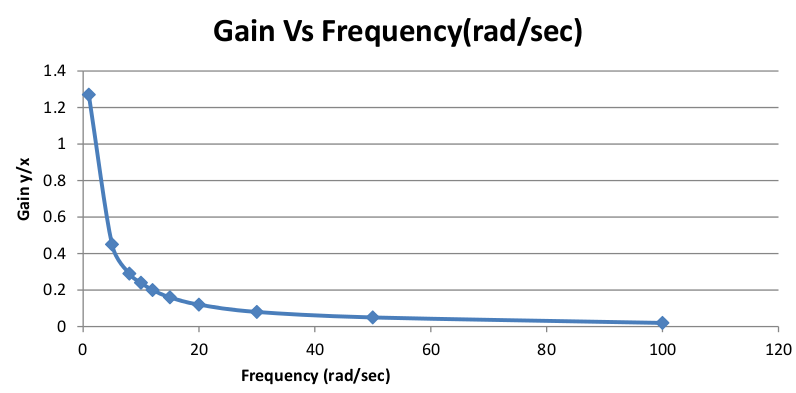
\includegraphics[width=0.7\textwidth]{gain_v_freq.png}
\end{align*}
\begin{align*}
\centering
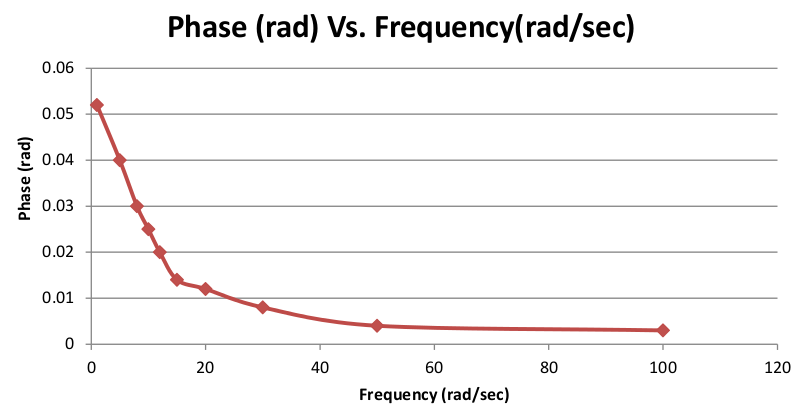
\includegraphics[width=0.7\textwidth]{phase_v_freq.png}
\end{align*}
\begin{itemize}
\item How does the system behaviour change with frequency?
\begin{itemize}
\item 
\end{itemize}
\end{itemize}
\subsubsection{Frequency Properties}
\begin{itemize}
\item Is the effect of the system the same at all frequencies?
\begin{itemize}
\item The effects of the system are visible the same at all frequencies.
\end{itemize}
\item How does the system behaviour change with frequency?
\begin{itemize}
\item The table of results was formed from setting the input amplitude at a constant value of 1, and the frequency was adjusted in order to allow us to measure the changes in amplitude of the output with different values of frequency. As we can see from the first graph, there appears to be an inverse relationship appearing between Gain and Frequency. For low values of frequency, the output amplitude was actually larger than the input, causing a gain value that was greater than 1. The graph begins to level off for higher frequencies, and seems to begin to approach a zero gain value. The proportion at which the gain decreases slows down as frequency is increased.
\end{itemize}
\end{itemize}
\subsubsection{Discussion}
\begin{itemize}
\item Discuss the significance of this plot with respect to the effect of system 1 on the Pulse Wave and Speech Signal.
\begin{itemize}
\item 
\end{itemize}
\end{itemize}

\section{Discussion}
\begin{enumerate}
\item What does frequency and phase mean with respect to a pure sinusoidal signal?
\begin{itemize}
\item Frequency refers to the number of oscillations per second that occur within the signal generated.
\item Phase shift refers to an offset through mathematics that is observed graphically by seeing a \emph{delay} in the signal from the phase $\phi$.
\end{itemize}
\item How does an LTI system affect a pure sinosoid?
\begin{itemize}
\item A sinosoidal input gives rise to a sinosoidal output with the same frequency. The amplitude however, is modified in the process.
\end{itemize}
\item What is the definition of an LTI system?
\begin{itemize}
\item An LTI system exhibits two behaviours:
\begin{itemize}
\item Time Invariance - The system must always behave the same between any two trials in time given that their starting conditions and inputs remain the same.
\item Additive Superposition - By exciting the system via input $H\{a_1x_1(t)+a_2x_2(t)\}$,the output should return $a_1y_1(t)+a_2y_2(t))$ through linearity.
\end{itemize}
\end{itemize}
\item What do the terms \emph{phase shift} and \emph{gain} mean?
\begin{itemize}
\item Phase Shift is a mathematical offset that is observed graphically by horizontal shifting through the characteristic equation $y=Asin(B(x-C))+D$ which can be applied to all trigonometric functions.
\item Gain is the ratio of the output with respect to the input. As it is unitless, it describes the factor at which a signal has been boosted or reduced with respect to its input.
\end{itemize}
\item How are the step and impulse response of system characterised?
\begin{itemize}
\item Step response is characterised through two key theorems within a given LTI system, \emph{Initial Value Theorem} and \emph{Final Value Theorem}, which correspond to the simplifications $y_\gamma(0^+)=H(\infty)$ and $y_\gamma(\infty)=H(0)$.
\item Impulse response is characterised through a short-duration time-domain signal. For continuous-time systems, this is the \emph{Dirac-delta function}, $\delta(t)$, while for discrete-time systems, this is the \emph{Kronecker-delta function}, $\delta[n]$; where $h(t)$ or $h[n]$ is defined as the output signal that results when an impulse is applied to the system's input, such that
$$x[n]=\sum^{\infty}_{k=0}x[k]\delta[n-k]$$
$$y[n]=\sum^{\infty}_{k=0}x[k]\delta[n-k]$$
\end{itemize}
\end{enumerate}

\section{Bibliography}
\begin{thebibliography}{3}
\bibitem{streetmanb}
  Ben G. Streetman \& Sanjay Kumar Banerjee,
  \emph{Solid State Electronic Devices, 6th edition},
  Prentice Hall (2006),
  Pages 154-388.
\end{thebibliography}
\end{document}
